\documentclass[a4paper]{article}
\usepackage[left=3cm, right=3cm, top=2cm, bottom=3cm]{geometry}

\usepackage{setspace}
\usepackage{listings}
\usepackage{authblk}
\usepackage{array}
\usepackage{tabularx}
\usepackage{multirow}
\usepackage[sort&compress]{natbib}
\usepackage[portuguese]{babel}
\usepackage[hidelinks]{hyperref}
\usepackage{xcolor}
\usepackage[inline]{enumitem}
\usepackage{amsmath}
\usepackage{mathtools}

\usepackage{tikz}
\usetikzlibrary{trees}

\usepackage{graphicx}
\usepackage{caption}
\usepackage{subcaption}
\graphicspath{ {./images/} }

\newlist{ilist}{enumerate*}{1}
\setlist[ilist]{label=(\arabic*)}

\begin{document}
\title{{\itshape Symbolic Regression}}
\author{Matheus Cândido Teixeira\thanks{matheuscandido2009@gmail.com}}
\affil{Departamento de Ciências da Computação - UFMG}
\maketitle

\section{Introdução}
A regressão simbólica (RS) é utilizada para resolver o problema de \emph{curve
fitting}. Para isso, um conjunto de amostras é fornecido, e o resultado é uma
função que possui o menor erro entre os pontos amostrados e o valor dela nesses
pontos.

Há diversos métodos de aplicar a regressão simbólica~\citep{jin2019}. Uma delas
é utilizando programação genética (GP, do inglês \textit{Genetic
  Programming})~\citep{poli2008}.  A GP é semelhante ao Algoritmo Genético (GA,
do inglês \textit{Genetic Algorithm}) no que tange os operadores genéticos, pois
ambos definem operadores de inicialização, seleção, cruzamento, mutação e
\textit{fitness}.

Na literatura, há diversas possíveis implementações dos operadores de GP. Por
exemplo, na fase de geração de indivíduos, que podem ser gerados utilizando o
método \textit{full} ou \textit{grow}. No primeiro método, o indivíduo é
complemente gerado, isto é, todos os seus nós são preenchidos, enquanto que no
último, não há essa necessidade. Na prática, é comum haver a combinação dos dois
métodos, denominado \textit{ramped half-and-half}~\citep{poli2008}, onde parte
da população é gerada usando um dos método e o restante utilizando o outro. A
seguir é apresentado as alternativas comuns para o desenvolvimento de cada
operador.

Os operadores de seleção são os mesmos dos utilizados em GA:
\textit{roulette~whell} e \textit{k-tournament}. O primeiro seleciona o
indivíduo com probabilidade proporcional a \textit{fitness} do indivíduo, ou
seja, se a fitness de um indivíduo for \emph{$f_k$} em uma população com $N$
indivíduos, a probabilidade dele ser selecionado é igual a $p(k) =
f_k/\sum_{i=0}^{N}f_i$. O outro método é o \textit{k-tournament}, que amostra
$k$ indivíduos aleatóriamente e seleciona o indivíduo com maior \textit{fitness}
nesse grupo. A diferença entre esses algoritmos está na pressão seletiva imposta
aos indivíduos. Porém \citet{poli2008} informa que o método
\textit{k-Tournament} é o mais comum.

O operador de cruzamento (ou \textit{crossover}) mais comum é denominado troca
de sub-árvore. Esse operador funciona da seguinte maneira: dois indivíduos
($I_1$ e $I_2$, respectivamente) são selecionados da população utilizando o
operador de seleção, após isso, para cada indivíduo, é escolhido um ponto
aleatório ($p_1$ e $p_2$) e um novo indivíduo é gerado pela junção da árvore
$I_1$ sem a sub-árvore com raíz no ponto $p_1$ com a sub-árvore extraida do
$I_2$ com raíz em $p_2$.

No caso do operador de mutação há diversas alternativas, entre elas estam a
mutação de um ponto e mutação de sub-árvore. O primeiro método, percorre todo o
indivíduo muda o gene com uma probabilidade $p_{op}$. O segundo método, seleciona
um ponto aleatório na árvore e, a partir desse ponto, uma sub-árvore é gerada
aleatóriamente. Note que no primeiro método há duas probabilidades envolvidas:
\begin{ilist}
\item a probabilidade de ocorrer mutação ($p_m$) e
\item a probabilidade de haver mutação em cada nó ($p_{op}$), caso o indivíduo
  tenha sido selecionado para mutação.
\end{ilist}

O último operador é o cálculo da \textit{fitness}. Como a regressão simbólica
busca minimizar o erro entre função gerada é os pontos amostrais, é comum
utilizar o erro (a diferença entre o ponto e o resultado da função nesse ponto)
como a forma de mensurar a adequação do indivíduo. Portanto, a \textit{fitness}
pode ser calculada como a somatória do erro absoluto (MAE), somatória do
quadrado do erro (MSE) ou raíz quadrada da somatória do quadrado do erro (RMSE)
entre a função gerado e os pontos amostrais fornecidos, onde as equações são
fornecidas a seguir:
\begin{align*}
  \textrm{MAE} &= \sum_{i}^{N}|y-\hat{y}| \\
  \textrm{MSE} &= \sum_{i}^{N}(y-\hat{y})^2 \\
  \textrm{RMSE} &= \sqrt{\sum_{i}^{N}(y-\hat{y})^2} = \sqrt{\textrm{MSE}}\\
\end{align*}

Outro aspecto importanto em GP é a representação dos indivíduos, que podem ser
representados linearmente ou em árvore. Ambas as representações possuem
vantagens, porém é mais comum a implementação em árvore. Juntamente com a
representação é importante definir os conjuntos de valores que eles podem
assumir. A escolha do conjunto de funções e operadores devem atender a três
restrições: Suficiência, Parcimônia e Fechamento~\footnote{Suficiência significa
que é possível expressar uma solução para o problema utilizando o conjunto de
operadores fornecido. Fechamento significa que os operadores devem suportar
todos os resultados dos demais. Parcimônia significa que o conjunto de
operadores não deve conter elementos desnecessários para representar os
indivíduos.}.

Por exemplo, para uma árvore com um conjunto de funções F:
$\{\sin(\cdot),\cos(\cdot)\}$ , com um conjunto de operadores $S: \{\times, + ,
-, \div\}$, uma possível árvore, cuja expressão é $\sin(ax^2)+\cos(by^2)$, onde
$a$ e $b$ são constantes numéricas e $x$ e $y$ são variáveis independentes, é:


\begin{center}
  \begin{tikzpicture}[level distance=.8cm,
      level 1/.style={sibling distance=4cm},
      level 2/.style={sibling distance=3cm},
      level 3/.style={sibling distance=2cm}]
    \node {+}
    child{node{$\sin$}
      child{node{$\times$}
        child{node{a}}        
        child{node{$\land$}
          child{node{x}}
          child{node{2}}
        }
      }
    }
    child{node{$\cos$}
      child{node{$\times$}
        child{node{b}}        
        child{node{$\land$}
          child{node{y}}
          child{node{2}}
        }
      }
    };  
  \end{tikzpicture}
\end{center}

Neste trabalho, o GP é utilizado para resolver o problema da RS. Os detalhes e
parâmetros da implementação são apresentados nas próximas seções. Para mensurar
a eficiência, o algoritmo é aplicado a 2 dataset, o primeiro é um dataset para
teste, que possui uma versão pura e outra com raídos aleatórios. O outro dataset
é um real e contém 8 colunas de \textit{features} e uma representando a
resposta.

O restante deste relatório é dividido em 3 seções: 
\begin{ilist}
\item A seção de metodologia apresenta os detalhes e escolhas de implementação
  e design de projeto.
\item A seção de experimentos apresenta os resultados obtidos do treinamento
  do algoritmo nos datasets.
\item Por fim, a seção de conclusão analisa os resultados obtidos da seção de
  experimentos.
\end{ilist}

\section{Metodologia} \label{sec:metodologia}
Nesta seção é descrito os datelhes de implementação e as decisões de design
aplicadas neste projeto. A descrição e detalhes são apresentados na ordem:
representação dos indivíduos, métodos de geração de indivíduos, métodos de
seleção, operador de crossover, operador de mutação, operador de reprodução,
eletismo e mecânismos de controle (ou de parada).

\subsection{Reprentação dos indivíduos} \label{subsec:representacao}
A representação dos indivíduos impacta diretamente na performance do sistema e
na expressividade dos invidívuos. Portanto, a princípio é apresentado como o
genótipo do indivíduo é definido e como ele é codificado.


Os indivíduos em GP são representados por árvores sintáticas, que possuem nós e
terminais. Os nós são operadores aritméticos ou funções e os terminais são
constantes ou variáveis. O conjunto de nós e terminais juntos formam o
\textit{primitive set} do GP~\citep{poli2008}. Neste sistema o conjunto de
funções são as funções trigonométricas ($\sin$, $\cos$ e $\tan$) e o logaritmo
com bases diferentes ($\log$ e $\log10$). Para a geração de constantes,
inicialmente foi testado o seguinte método: gerar valores aleatórios utilizando
uma distribuição multimodal. A escolha desse método se deve ao fato que muitas
funções matemáticas possuem contantes no intervalo $[-1, +1]$, porém os
resultados iniciais demonstraram que essa abordagem era problemática pois muitos
valores de dimensões não proporcionais ao do dataset eram geradas. Para contorna
esse problema, foi adotado uma abordagem mais simples: gerar constantes
aleatóriamente no intervalo de 0 a 255 e o fenótipo é igual a $-10+20/256\cdot
\texttt{constante}$, ou seja, um valor real no intervalo $[-10, 10)$.  As
  variáveis são geradas aleatóriamente, onde um número inteiro no intervalo $(0,
  N]$, onde $N$ deve ser menor ou igual ao número de colunas do dateset menos
um, ou seja, se há 10 colunas de \textit{features} e uma que representa a
variável de resposta, então $N$ deve ser igual ao número de \textit{features} ou
menor.

Outro aspecto importante na representação dos indivíduos é que eles são
geralmente representados por uma estrutura de árvore. A literatura define
diversas estruturas de árvores, como árvores binárias, B-\textit{tree}, entre
outras. Um problema na representação utilizando esses tipos de árvores é a
indireção, que pode afetar a performance do sistema~\citep{faria2013}, portanto,
para evitar os efeitos da indireção de ponteiros, os indivíduos são
representados utilizando \textit{Heaps}, que são árvores especializadas. Nesse
tipo de estrutura, os ponteiro são implicitamente substituídos por índices. O nó
à esquerda está na posição $2n+1$ do vetor e o nó à direita está na posição $2n
+ 2$. Outra vantagem no uso de \textit{Heaps} está no fato dos dados serem
armazenados linearmente, o que reduz os efeitos do \textit{cache miss}, causado
por dados espalhados na memória.

O sistema é flexível na escolha da profundidade máxima que um indivíduo
(representado por uma árvore) possui e permite ao usuário especificar qualquer
profundidade aos indivíduos.  Um fator que pode ser vantajoso é que o espaço
ocupado por um indivíduo é determinístico, ou seja, se a profundidade for de
$l$, então a quantidade de nós nessa profundidade é $2^l$.  A quantidade total
de nós que um indivíduo possui é igual a $\sum_{l=0}^{L}2^l=2^{L}-1$, onde $L$ é
a profundidade máxima da árvore. Portanto, para uma população com $N$ indivíduos
e profundidade máxima $L$, há $N\times(2^{L}-1)\times\texttt{sizeof(nó)}$ bytes
ocupados.

Em conclusão, os indivíduos são representados como árvore no ponto de vista
semântico e como vetor contíguo na memória.  Espera-se que com essa estrutura
haja um ganho na performance devido a redução dos efeitos da indireção e por
conseguência de \textit{cache miss}.

\subsection{Operadores de Geração} \label{subsec:generation}

A literatura de define vários operadores de geração de indivíduos, como o método
\textit{Full}, \textit{Grow} e a combinação de ambos, denominado \textit{Ramped
  Half-and-Half}. O método \textit{Full}, gerada um indivíduo preenchendo todos
os seus nós. O método \textit{Grow}, em contraste com o método anterior,
preenche um usuário não necessariamente preenchendo todos os nós. Por fim, o
último método gera individuos utilizando os dois métodos anteriores, com 50\% de
probabilidade para ambos~\citep{poli2008}.

Nessa implementação, há suporte para os três tipos de geração. O método
\textit{Full} é gerado iterativamente, preenchendo os $L-1$ niveis da árvore do
indívido com funções ou operadores e a última camada com terminais (constantes
ou variáveis).  O método \textit{Grow} é gerado com uma função recursiva, que
escolhe um operador ou função como raíz e utiliza uma função de distribuição
uniforme para decidir se avança ou não mais um nível em cada ramo da árvore,
isto é, o filho à esquerda ou à direita. Já o método \textit{Ramped
  Half-and-Half} utiliza também uma função de distruibuição uniforme para
decidir qual dos dois métodos utilizar.

\subsection{Operadores de Seleção} \label{subsec:selection}

Dois operadores de seleção que são frequentemente utilizados são o
\textit{Roulette Wheel} e o \textit{k-Tournament}. O primeiro método seleciona
algum indivíduo da população com probabilidade proporcional a sua
\textit{fitness}, isto é, $p(i)=f_i/\sum_{k=0}^{N}f_k$. Já o último método
amostra \textit{k} indivíduos aleatoriamente e seleciona o indivíduo que possui
a maior \textit{fitness} dessa amostragem. O método \textit{Tournament} possui
a vantagem de permitir o ajuste da pressão seletiva aplicada, onde valores
menores de $k$ geram baixa pressão seletiva ao passo que grandes valores de $k$
aumentam a pressão seletiva~\citep{Baeck1994}.

Na aplicação desenvolvida é possível utilizar ambos os métodos de seleção. Para
o \textit{k-Tournament} também é possível especificar o valor de \textit{k}.
Essa flexibilidade facilita os testes e a escolha do valor adequado para o
parâmetro, que ajusta a pressão seletiva da seleção e, assim, na interfere na
convergência da população.

\subsection{Operadores de \textit{Crossover}} \label{subsec:crossover}

A operação de \textit{crossover} utiliza o \hyperref[subsec:selection]{operador
  de seleção} para a escolha de dois indivíduos para que eles possam
reproduzir. A reprodução depende de dois fatores: a probabilidade de
\textit{crossover} ($p_c$) e o método de \textit{crossover}.  Uma método comum
para realizar esse evento é denominado troca de sub-árvore, onde duas árvores
são selecionadas utilizando os operadores de seleção e para cada árvore um ponto
é selecionado aleatóriamente. Para uma árvore, o pai, a sub-árvore com raíz no
ponto selecionado é removido e no lugar é inserido a sub-árvore com raíz no
ponto selecionado na outra árvore, a mãe. A escolha do ponto que determina a
raíz da sub-árvore é feaita aleatóriamente, porém , na implementação do
algoritmo, a escolha desses pontos é feita de tal modo que a soma da
profundidade da árvore pai da raíz até o ponto selecionado com a profundidade da
sub-árvore oriunda dá árvore mãe não seja maior de que o comprimento máximo que
um indivíduo pode possuir.

No que tange a implementação, o parâmetro $p_c$ pode assumir qualquer valor no
intervalo $(0, 1)$. A decisão desse parâmetro pode alterar o valor dos
\hyperref[subsec:mutation]{operadores de mutação} ($p_m$) e do
\hyperref[subsec:reproduction]{operador de reprodução} ($p_r$). A forma como a
probabilidade deles pode ser ajustada automaticamente em situações específicas é
descrito na seção \nameref{subsec:smart_par}.

\subsection{Operadores de Mutação} \label{subsec:mutation}

A literatura define os operadores de dois tipos de operadores de mutação:
mutação de sub-árvore e \textit{one-point mutation} (OPM)~\citep{poli2008}. No
primeiro método um ponto é escolhido aleatóriamente na árvore e, a partir desse
ponto, uma sub-árvore é gerada aleatóriamente. No algoritmo implementado, o
método de geração da sub-árvore é o mesmo empregado no método \textit{grow} de
geração (veja Seção \ref{subsec:generation}). O outro método de mutação é o
OPM. Esse método é aplicado sobre todos os nós e terminais da árvore do
indivíduo, onde há a probabilidade de $p_op$ de haver mutação nesse nó. A
mutação em um nó específico ocorre alterando o elemento contido nele por outro
da mesma classe, por exemplo, em um nó contendo a função $\sin$, a OPM pode
alterá-lo para $\tan$, ou seja, manteve a classe (uma função), porém alterou o
elemento contido no nó.

Na implementação, ambos os métodos possuem igual probabilidade de serem
empregados (50\%-50\%, respectivamente), porém no caso do OPM a probabilidade de
mutação de cada nós é especificado separadamente e é possível controlar o valor
dessa probabilidade através da constante $p_op$, que controla a probabilidade de
OPM.

\subsection{Operador de Reprodução} \label{subsec:reproduction}

Quando a probabilidade de \textit{crossover} e de mutação somadas é menor do que
100\%, algebricamente expresso por $p_c + p_m < 1$, entra em ação o operador
de reprodução, que basicamente seleciona indivíduos da população utilizando
o operador de seleção selecionado até que a próxima geração atinja o tamanho
máximo da população.

Esse parâmetro pode ser ajustado na aplicação através do parâmetro $p_r$, e,
dessa forma, os operadores de mutação ($p_m$) e de \textit{crossover} ($p_c$)
são ajustados automaticamente.

\subsection{Eletismo}

Após a geração da próxima geração de indivíduos há duas possibilidades:
descartar a população anterior ou manter os indivíduos da população anterior
com a nova população e selecionar os que possuem maior \textit{fitness} em ambas
as populações. Essa última abordagem é denominada eletismo.

O sistema desenvolvido permite que a aplicação do eletismo seja controlado pelo
parâmetro, que indica se deve ou não ocorrer eletismo.

\subsection{\textit{Fitness}}

A \textit{Fitness} determina o quão adaptado um indivíduo está e é utilizada
para comparação entre os indivíduos. A função para calcular a \textit{fitness}
está relacionada ao problema, e, no caso da RS, algumas formas de mensurar a
\textit{fitness} de um indivíduos são o erro médio absoluto (MAE), o error médio
quadrado (MSE) e a raiz do erro médio quadrado (RMSE). Independente da métrica
utilizada para calcular a \textit{fitness}, o objetivo é minimizar o erro.

Na implementação desenvolvida todas as três métricas descritas estão disponíveis
e fica a critério do usuário a escolha de qual métrica de erro utilizar.

\subsection{Ajuste Inteligente de Parâmetros}\label{subsec:smart_par}

As probabilidades de \textit{crossover} ($p_c$), de mutação ($p_m$) e de
reprodução ($p_r$) estão relacionadas através da seguinte equação:
\begin{equation} \label{eq:prob_stability}
  p_c + p_m + p_r = 1
\end{equation}
Geralmente, é comum atribuir valores altos para $p_c$ e mais baixos $p_m$, porém
quando eles não somam a 1, o operador de reprodução $p_r$ é atribuido ao
complemento, de tal forma que a equação \ref{eq:prob_stability} é satisfeita.

Outra forma de controle ocorre quando o usuário atribui um valor para $p_r$,
neste caso, os valores de $p_c$ e $p_m$ são ajustado para que a soma deles
resulte em $1-p_r$. Quando isso ocorre, a proporção relativa entre eles é
mantida, isto é:

\noindent\begin{minipage}{.5\linewidth}
  \begin{equation*}
    p_c = \frac{p_c}{p_c+p_m}\times (1-p_r)  
  \end{equation*}
\end{minipage}
\begin{minipage}{.5\linewidth}
  \begin{equation*}
    p_m = \frac{p_m}{p_c+p_m}\times (1-p_r)  
  \end{equation*}
\end{minipage}

\subsection{Ambiente para Testes}

Devido ao fato da GP tomar decisões aleatóriamente, o resultado pode variar
entre execuções. Para alcançar um grau de confiança nos resultados obtidos, é
necessário repetir os testes diversas vezes. Para isso, o sistema implementado
possui suporte para testes.

Para testar os alguns parâmetro o usuário deve fornecer um arquivo
\texttt{*.csv}, onde cada linha deve conter uma lista de números inteiros que
são utilizados como \textit{seeds} para o geradores de números aleatórios. O
gerador utilizado na implementação é o \texttt{32-bit Mersenne Twister}. Os
testes são repetidos para cada linha contida no arquivo contendo as
\textit{seeds}.

Após a bateria de testes, o sistema retorna um relatório contendo a média e o
desvio padrão das seguintes estatísticas de cada geração: menor, maior, média,
mediana, desvio padrão, variância da \textit{fitness} da população, quantidade
de indivíduos melhores que a média da população anterior e a quantidade de
indivíduos únicos na população. Esse relatório pode ser salvo em um arquivo
\texttt{*.csv}, caso o usuário forneça o nome do arquivo de destino através da
opção \texttt{-o [nome-do-arquivo]}.

\subsection{Desempenho}

Conforme mencionado nas seções anteriores, as escolhas da representação dos
indivíduos foi feita tendo em vista a performance do sistema. Um fator a ser
explorado é a performance do sistema com a introdução de paralelismo.

\subsection{Compilação}
A implementação do algoritmo foi feita em \texttt{C++}. A compilação pode ser
complexa devido a quantidade de dependêcias em bibliotecas para leitura de
arquivos \texttt{*.csv} e \textit{parser} dos argumentos. Para contornar essa
complexidade, o CMake foi utilizado para gerar o projeto de modo que o sistema
utilize o compilador \texttt{C++} disponível no sistema. Outro aspecto
importante é que o código depende da \textit{standard} 17 da linguagem, portanto
é necessário que o compilador ofereça suporte a essa especificação da
linguagem. O sistema foi testado utilizando os compiladores GNU GCC 10.0.1 e o
MSVC19, ambos os compiladores foram capazes de compilar o sistema. Os comandos
necessários para compilar e executar o programa no Linux ou Windows podem ser
vistos no \hyperref[lst:code_1]{Código~\ref*{lst:code_1}} ou
\hyperref[lst:code_2]{Código~\ref*{lst:code_2}}, respectivamente.

\begin{lstlisting}[language=bash, caption={Comandos para compilar no Linux},
    label={lst:code_1}, frame=shadowbox, frameround=fttt]
  mkdir bin && cd bin    
  cmake .. && cmake --build .  
  cd src           
  ./sreg [parametros]
\end{lstlisting}

\begin{lstlisting}[language=bash, caption={Comandos para compilar no Windows},
    label={lst:code_2}, frame=shadowbox, frameround=fttt]
  mkdir bin 
  cd bin    
  cmake ..  
  cmake --build .  
  cd src/Debug/           
  sreg.exe [parametros]
\end{lstlisting}

Os parâmetros que o sistema suporta são apresentados na
\hyperref[tbl:parameters]{Tabela~\ref*{tbl:parameters}}. Os parâmetros que não
possuem argumentos são aqueles que aceitam um intervalo númerico (inteiro ou
real), não necessitam de argumentos ou aceitam uma string, como nome de arquivo,
por exemplo.


\noindent\begin{table}[h]
  \center
  \caption{Parâmetros do Sistema}
  \label{tbl:parameters}
  \begin{tabular}{|c|r|p{1.8cm}|r|}
    \hline
    Parâmetro & Comando & Argumentos & Exemplo \\ \hline
    Arquivo de entrada & 1º parâmetro & & \texttt{./sreg ../data/concrete.csv}\\ \hline
    Ajuda & \texttt{-h}, \texttt{--help} & & \texttt{-h} \\ \hline
    Relatório & \texttt{-o}, \texttt{--output} & & \texttt{-o report.csv} \\ \hline
    \# de variáveis & \texttt{-n}, \texttt{--variables} & & \texttt{-n 8} \\ \hline
    Tamanho da população & \texttt{--population-size} & & \texttt{--population-size 500} \\ \hline
    Limite de gerações & \texttt{--max-generation} & & \texttt{--max-generation 100} \\ \hline
    Método de geração & \texttt{--generation-method} & ramped-hh, full, grow & \texttt{--generation-method ramped-hh} \\ \hline
    Profundidade da árvore & \texttt{--max-depth} & & \texttt{--max-depth 7} \\ \hline
    Método de seleção & \texttt{--selection-method} & roulette, tournament & \texttt{--selection-method tournament} \\ \hline
    k (tamanho do torneio) & \texttt{-k}, \texttt{--k-tournament} & & \texttt{-k 7} \\ \hline
    Prob. \textit{crossover} & \texttt{-pc}, \texttt{--prob-crossover} & & \texttt{-pc 0.9} \\ \hline
    Prob. mutação & \texttt{-pm}, \texttt{--prob-mutation} & & \texttt{-pm 0.05} \\ \hline
    Métrica de erro & \texttt{--error-metric} & mae, mse, rmse & \texttt{--error-metric rmse} \\ \hline
    \textit{Fitness threshold} & \texttt{--fitness-threshold} & & \texttt{--fitness-threshold 0.001} \\ \hline
    Eletismo  & \texttt{-E}, \texttt{--eletism} & & \texttt{-E} \\ \hline
    Seeds & \texttt{--seeds} & & \texttt{--seeds ../data/seeds.csv} \\ \hline
  \end{tabular}
\end{table}

\section{Experimentos}
Nesta seção é apresentado resultados dos experimentos realizados. Os resultados
apresentados são estatísticas geradas a partir da execução do sistema diversas
vezes alterando as \textit{seeds} do gerador pseudo-aleatório. São fornecidos
para o teste 31 sementes, cada uma contendo 20 números inteiros gerados
aleatóriamente.  Ao aplicar o mesmo conjunto de sementes, os resultados devem
ser reproduzíveis.

\subsection{Dataset Experiamental}
Este dataset possui uma versão sem ruído e uma versão ruidosa de uma função
matemática desconhecida. O algoritmo será aplicado em ambas as versões. Esse
dataset foi escolhido pois simula um fenômeno físico hipotético, no qual a
regressão simbólica pode ser aplicada para gerar uma função algébrica para ele.

O primeiro teste tem o objetivo de identificar qual o tamanho da população que
atinge o melhor valor de \textit{fitness} em média. Para isso, o tamanho da
população é variado e os demais parâmetros são mantidos constantes. Os valores
testados variam de uma população pequena (50 indivíduos) até uma população
grande (500 indivíduos). Os resultados estam presentes na
\hyperref[fig:sr_div_pop_sz]{Figura~\ref*{fig:sr_div_pop_sz}}, onde é possível
verificar que a qualidade da \textit{fitness} aumenta proporcinalmente em
relação ao tamanho da população. Como cada indivíduo evolui de modo
independente, o espaço de soluções é explorado conforme a quantidade de
indivíduos aumenta, fato que é demonstrado na figura. Pelo fato da população
com 500 indivíduos ter a melhor solução, os próximos testes tem o tamanho da
população fixa em 500 indivíduos.

Os próximos parâmetros a serem variados são a probabilidade de
\textit{crossover} e de mutação. Como os eles estão diretamente relacionados,
eles devem ser variados de modo proporcional. Esses parâmetros têm impacto na
\textit{exploration} e \textit{explotation} da solução. O \textit{crossover} faz
com que as melhores soluções sejam combinadas para gerar soluções aperfeiçoadas,
enquanto que a mutação faz que novos indivíduos sejam gerados, trazendo novidade
para a população. No caso do GP, o \textit{crossover} tem impacto semelhante ao
da mutação, pois não há contexto envolvido, o que faz que os indivíduos não
necessariamente leve a indivíduos melhores que os pais. A
\hyperref[fig:sr_div_pc_pm]{Figura~\ref*{fig:sr_div_pc_pm}} demonstra esse
efeito. A população gerada com a probabilidade de \textit{crossover} mais
elevada atige máximos locais e permanece neles, enquanto que as populaçõeos com
maior taxa de mutação explora novas soluções com maior frequência e,
eventualmente, encontra soluções melhores. Com base nos resultados obtidos, os
próximos experimentos são realizados mantendo-se $p_c=60\%$ e $p_m=30\%$.


Outro aspecto importante é a pressão seletiva imposta à população. Uma das
formas de controlar a pressão seletiva é configurando o método de seleção. Para
o caso do método $k$-\textit{tournament}, a pressão seletiva pode ser controlada
através do parâmetro $k$, que representa a quantidade de indivíduos que são
selecionados para o torneio, onde o indivíduo que possui a melhor
\textit{fitness} (a maior para um problema o maximização ou a menor para um
problema de minimização) é retornado. Os valores maiores de $k$ aumentam a
pressão seletiva, pois a probabilidade dos indivíduos que possuem valoers
maiores de \textit{fitness} serem selecionados é maior, e, consequentemente,
indivíduos com \textit{fitness} menores tem menor probabilidade de serem
selecionados para cruzamento. A consequência disso é que há a possíbilidade de
indíviduos que atinjam máximos/mínimos locais sejam selecionados com maior
frequência e levem a população para uma convergência prematura para um ótimo
local. Os efeitos da variação do parâmetro $k$ na população pode ser visto na
\hyperref[fig:sr_div_k]{Figura~\ref*{fig:sr_div_k}}. Como a figura indica, as
populações como o tamanho do torneio maior possuem uma queda da \textit{fitness}
abrupta no começo, porém estagnam com o passar das gerações, pois indivíduos que
atingem máximos locais dominam a população e exploram as melhores soluções já
encontradas ao invés de buscar novas. Por outro lado, a população com o tamanho
do torneio pequeno tem a convergência inicial baixa, porém ao explorar o espaço
de soluções entra soluções melhores do que as soluções encontradas em população
com o tamanho do torneio grande. Um fator importante a ser considerado é que o
eletismo está ativado, portanto más soluções não têm grande impacto na melhor
solução, porém sem eletismo o tamanho do torneio pode levar a populações que não
convirjam devido a baixa pressão seletiva. Para os demais teste, o tamanho do
torneio é mantido em $k=3$.

O último parâmetro explorado é o efeito do eletismo que pode afetar a
convergência ou não da população conforme mencionado acima. O eletismo evita que
soluções boas sejam perdidas e garante que elas serão mantidas caso novas
soluções melhores do que as atuais não sejam encontradas, porém pode levar a
convergência pematura, uma vez que soluções ótimas locais são mantidas e pouco
espaço é dado a novas soluções. Os resultados da presença do eletismo na
população fica evidente analisando a \textit{fitness} da população com e sem o
efeito do eletismo, conforme apresentado na
\hyperref[fig:sr_div_eletism]{Figura~\ref*{fig:sr_div_eletism}}. Na figura é
possível ver que sem o eletismo, não há convergência. Esse efeito está
relacionado a baixa pressão seletiva do parâmetro $k$ do método de seleção, pois
a pressão seletiva é baixa e soluções ótimas encontradas durante a exploração do
espaço de busca não são mantidas na população.

\begin{figure}[h]
  \caption{Resultados da \textit{fitness}}
  \label{fig:sr_div_fitness}
  \begin{subfigure}[t]{0.5\textwidth}
      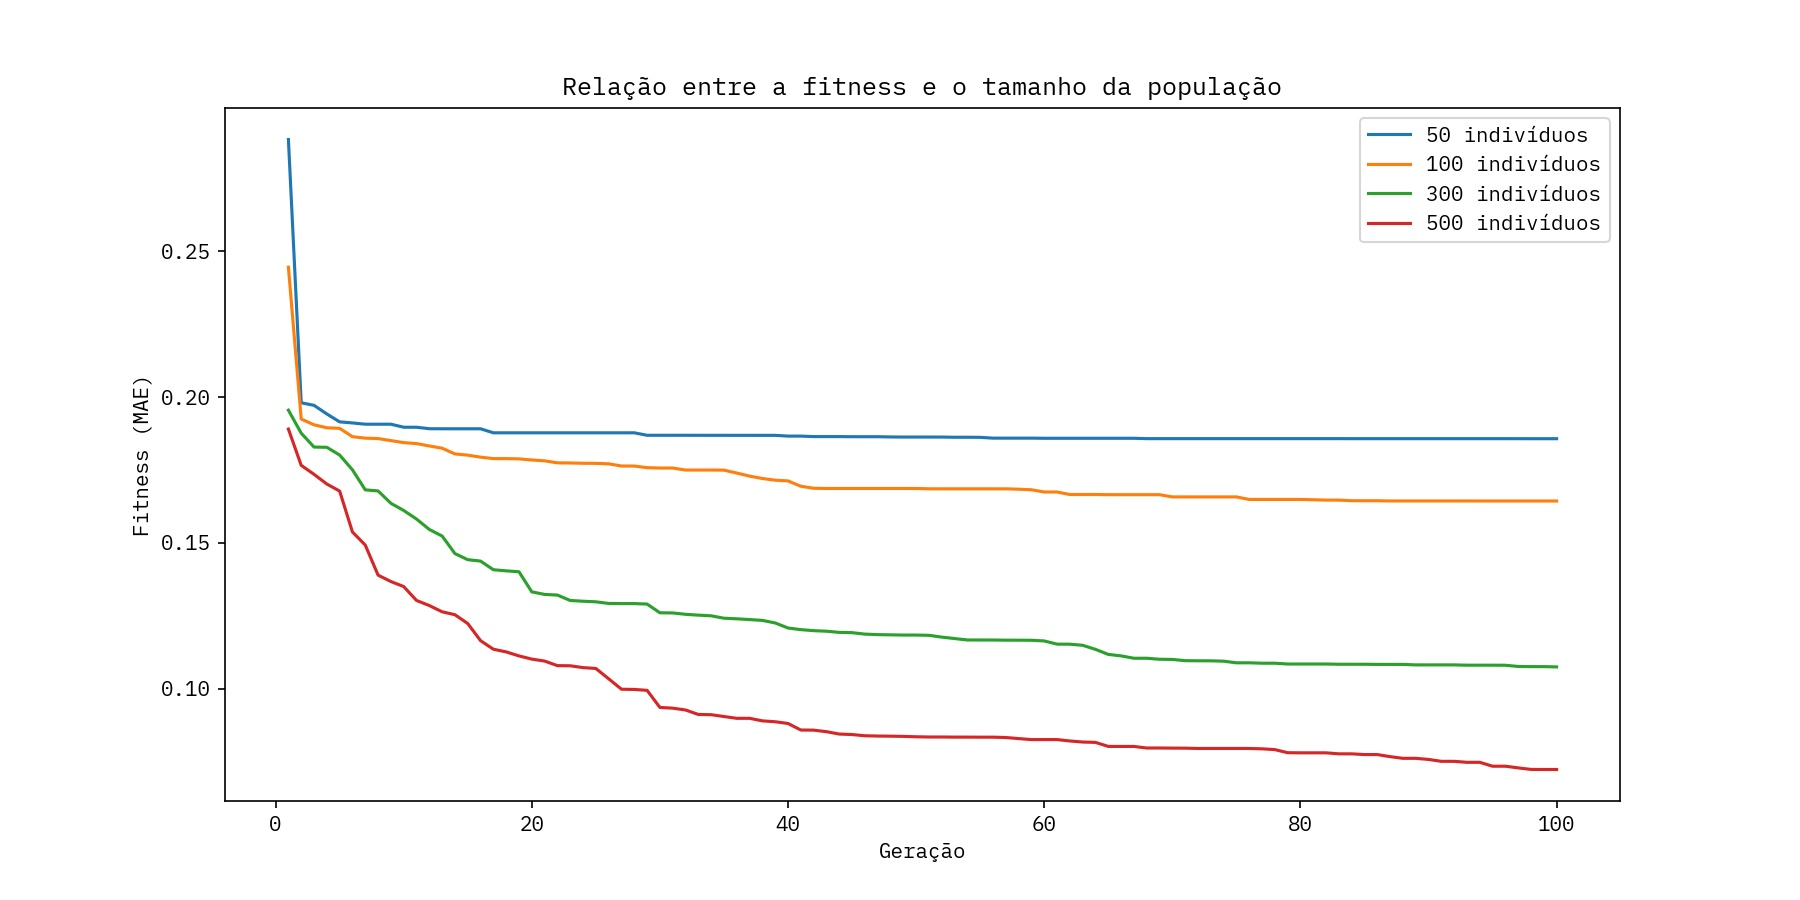
\includegraphics[width=\textwidth]{sr_div_pop_sz}
      \caption{Tamanho da população}
      \label{fig:sr_div_pop_sz}
    \end{subfigure}
    \begin{subfigure}[t]{0.5\textwidth}
      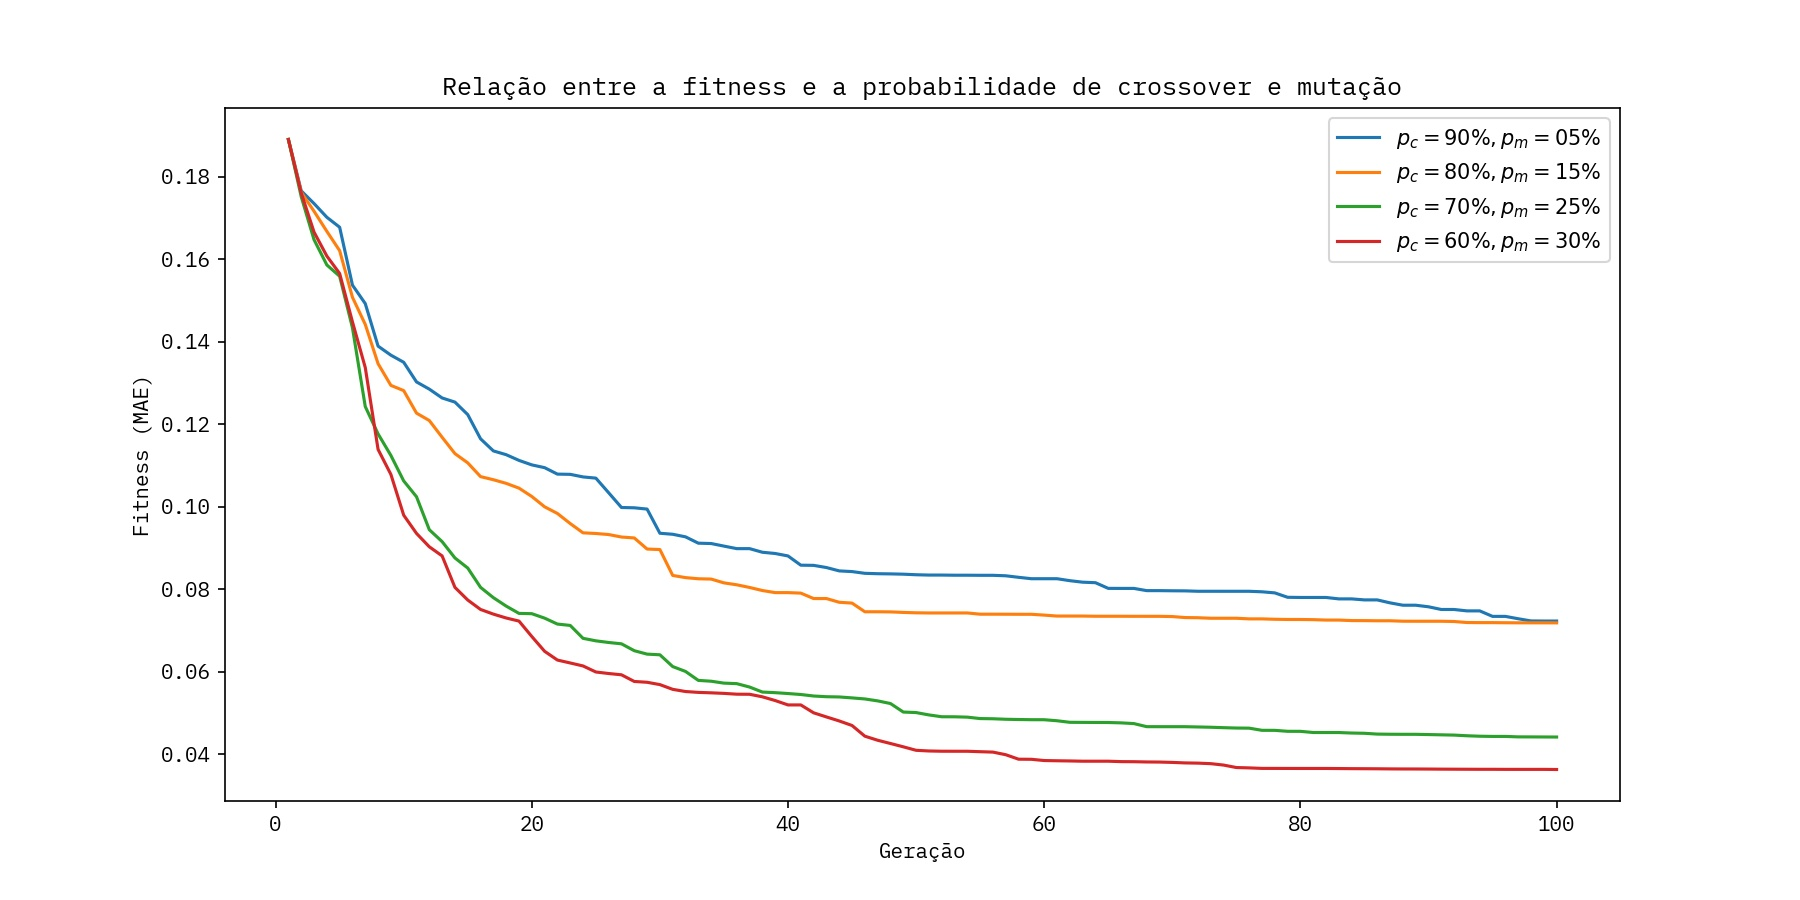
\includegraphics[width=\textwidth]{sr_div_pc_pm}
      \caption{Probabilidade de \textit{crossover} e mutação}
      \label{fig:sr_div_pc_pm}
    \end{subfigure}
    \begin{subfigure}[t]{0.5\textwidth}
      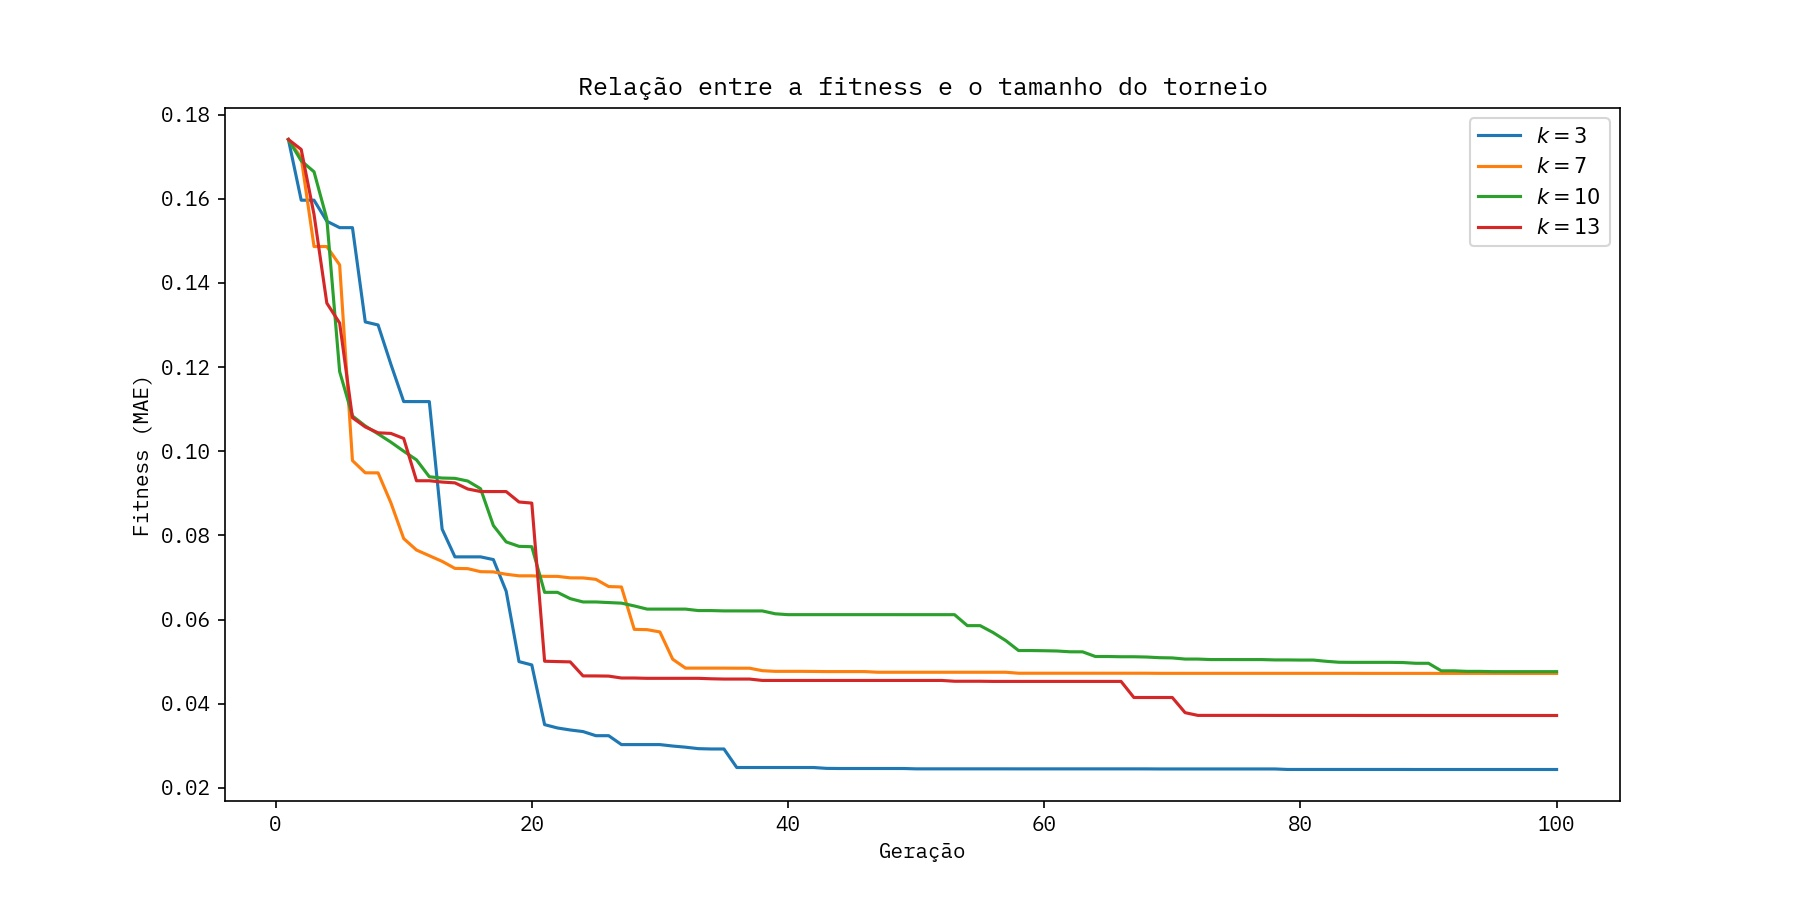
\includegraphics[width=\textwidth]{sr_div_k}
      \caption{Tamanho do torneio}
      \label{fig:sr_div_k}
    \end{subfigure}
    \begin{subfigure}[t]{0.5\textwidth}
      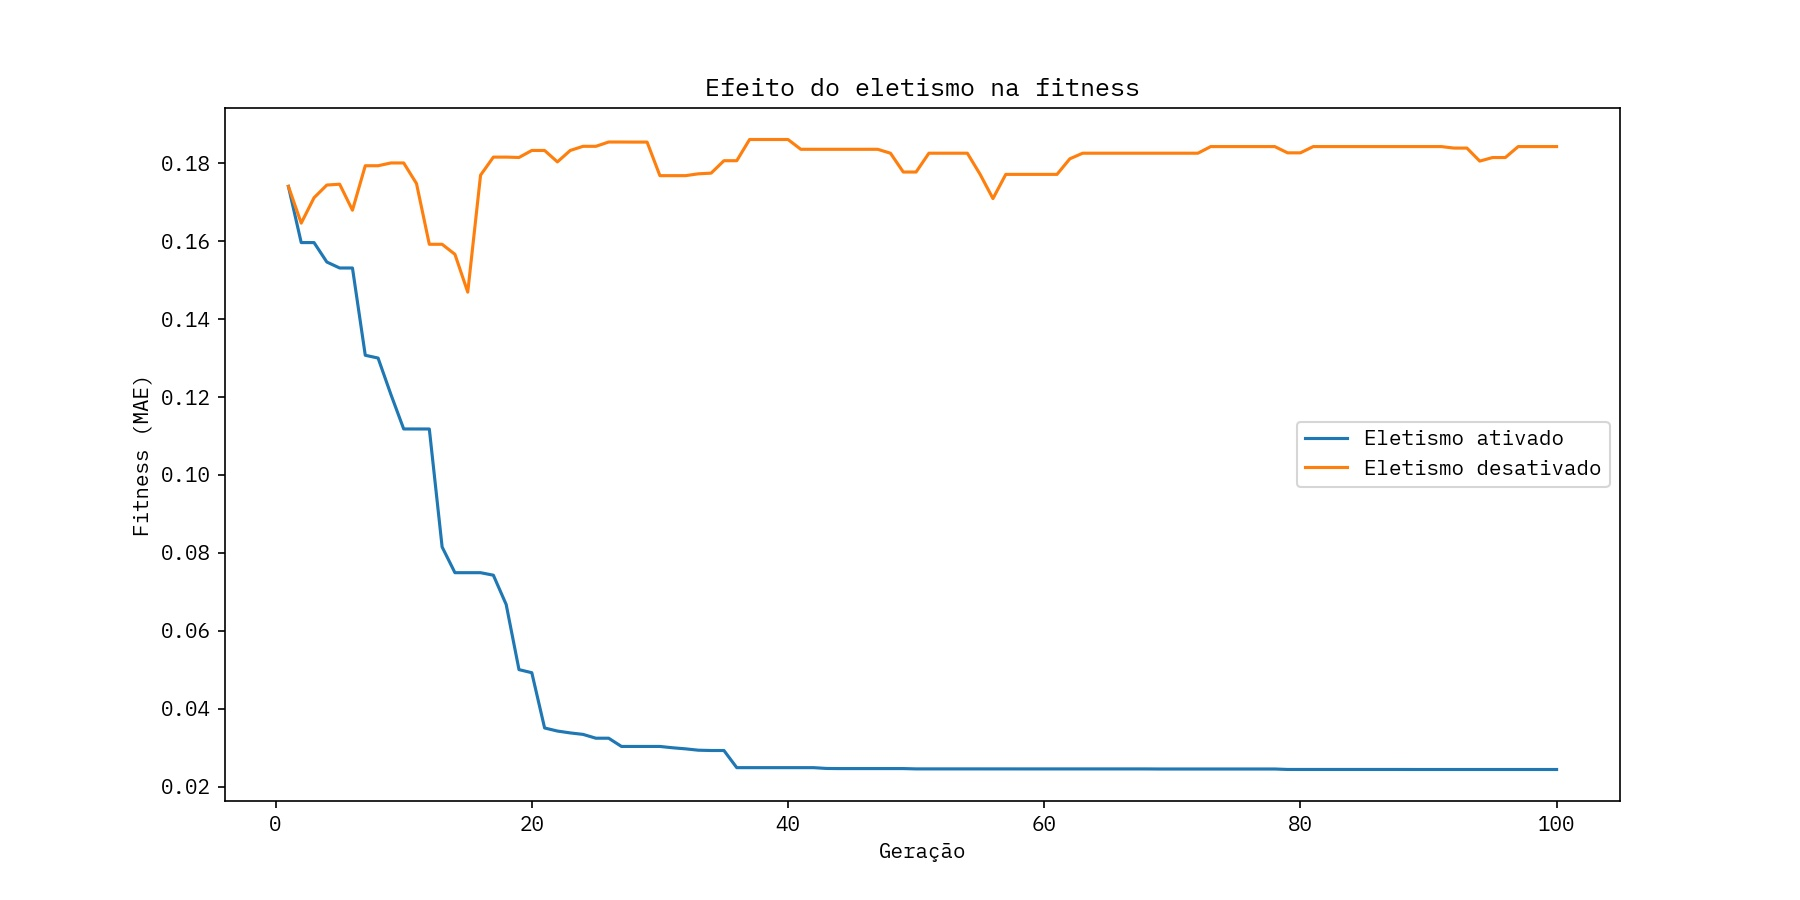
\includegraphics[width=\textwidth]{sr_div_eletism}
      \caption{Efeito do eletismo}
      \label{fig:sr_div_eletism}
    \end{subfigure}
\end{figure}

Agora, para verificar a robustez do sistema, a mesma abordagem é aplicada ao
dataset com ruído para verificar a capacidade de adaptação do algoritmo. Os
resultados são semelhantes aos obtidos no dataset sem ruídos até a seleção do
parâmetro $k$, onde o torneio muito pequeno faz com que a população não
convirja. O valor do torneio que retornou atingiu o melhor valor para a
\textit{fitness} foi $k=7$. Outro teste feito foi do efeito do eletismo na
população e os resultados indicam que a presença ou ausência do eletismo não
altera significativamente a \textit{fitness} da população, isso se deve ao
tamanho do torneio, que gera um aumento da pressão seletiva entre os indivíduos
independente da presença de eletismo. A
\hyperref[fig:noise]{Figura~\ref*{fig:noise}} apresenta esses resultados.

\begin{figure}[h]
  \caption{Resultados para o dataset com ruídos}
  \label{fig:noise}
  \begin{subfigure}[t]{0.5\textwidth}
    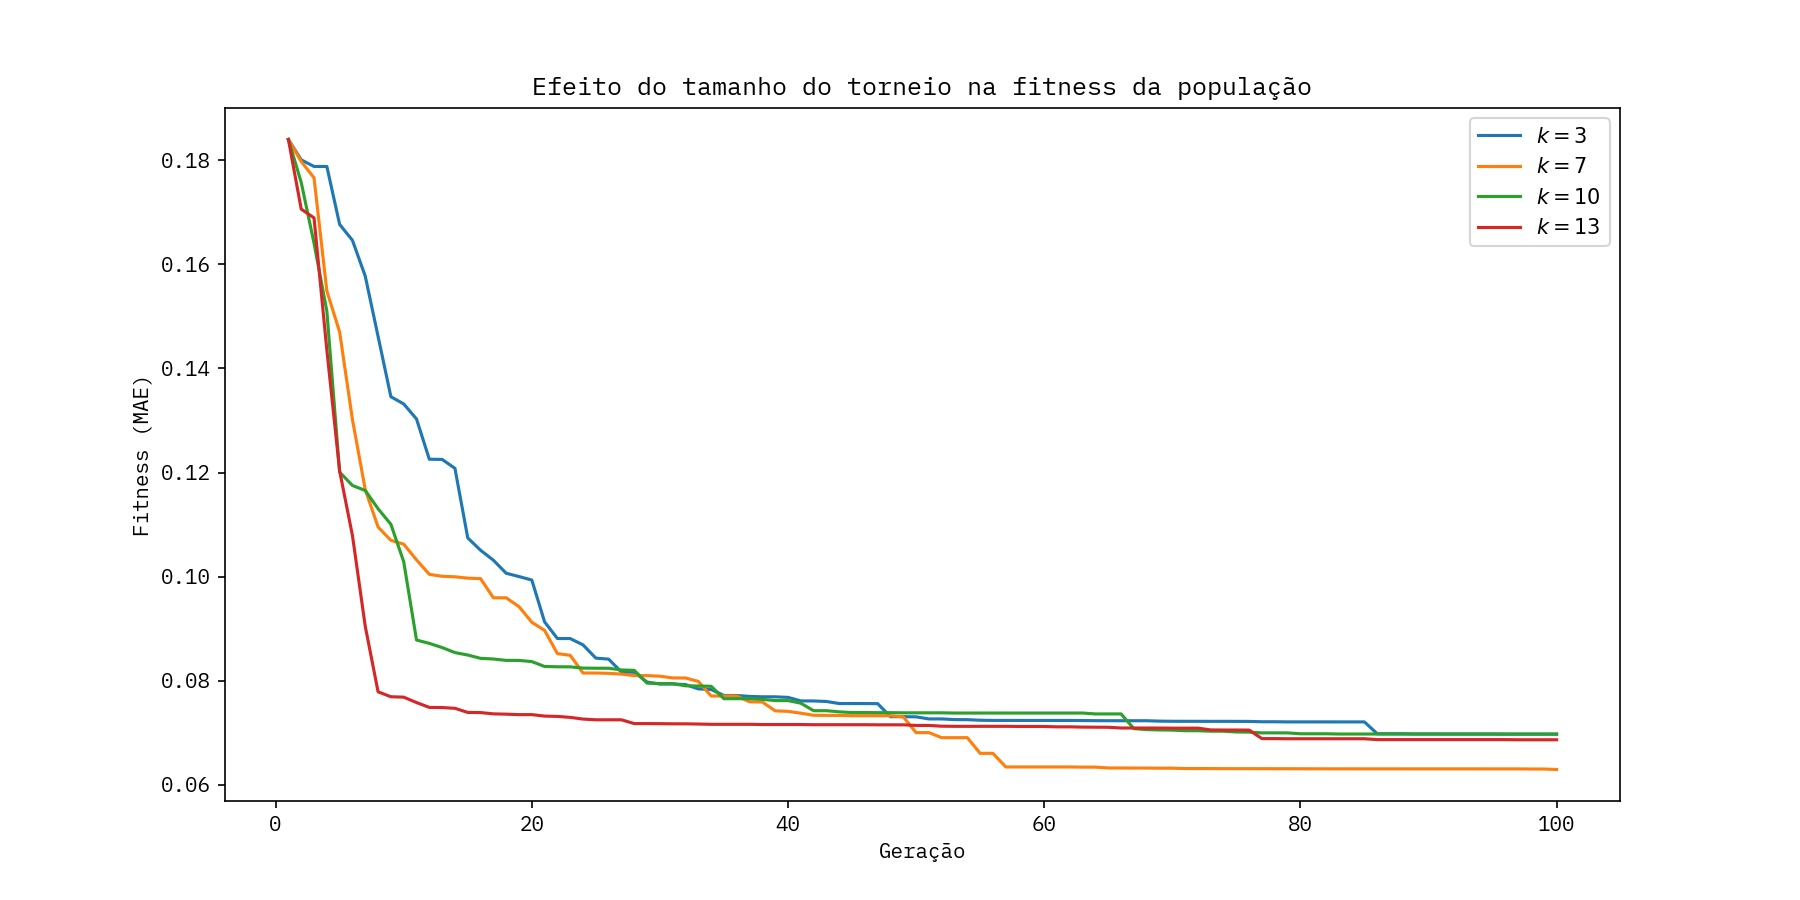
\includegraphics[width=\textwidth]{sr_noise_k}
    \caption{Efeito do tamanho do torneio na população}
    \label{fig:noise_k}
  \end{subfigure}
  \begin{subfigure}[t]{0.5\textwidth}
    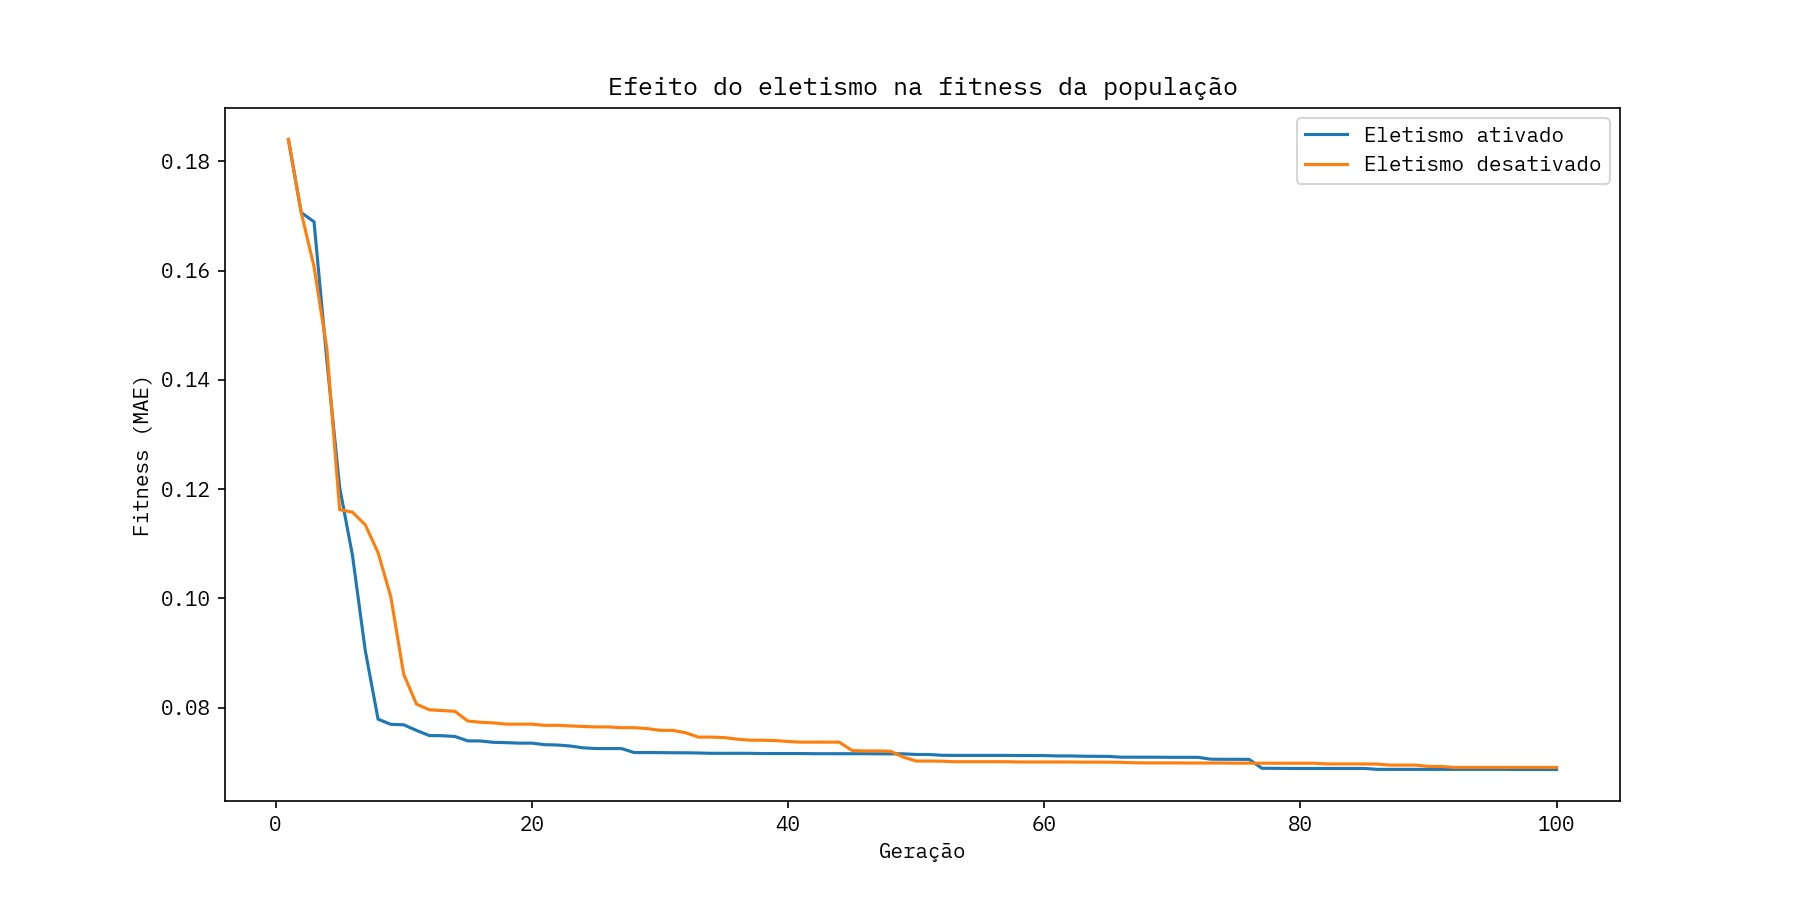
\includegraphics[width=\textwidth]{sr_noise_eletism}
    \caption{Efeito do eletismo na população}
    \label{fig:noise_eletism}
  \end{subfigure}
\end{figure}

Um exemplo de solução gerada para o dataset com ruídos (direita) e sem ruídos
(esquerda) pelo algoritmo pode ser vista abaixo, onde o erro médio absoluto foi
de $0.0352019$ e $0.000256972$, respectivamente:

\noindent\begin{minipage}[t]{0.5\textwidth}
\begin{equation*}
\frac{\frac{\frac{1}{x+x}}{3.046875}+\frac{1}{(7.5-x-5.625/x)}}{4.453125-(\sqrt{\sqrt{x}}-(\sqrt{5.234375}+\frac{1}{7.5}))}+x
\end{equation*}
\end{minipage}
\begin{minipage}[t]{0.5\textwidth}
  \begin{equation*}
    x+\frac{\frac{\frac{1}{x}\cdot\frac{1}{-7.1875}}{\frac{1}{7.109375^{-2.890625}}}-(\frac{1}{x}\cdot\frac{1}{-8.359375})\cdot\frac{1}{x/x}}{4.765625}
  \end{equation*}
\end{minipage}
\vspace{0.5cm}


A \hyperref[fig:best_sdn]{Figura~\ref*{fig:best_sdn}} demostra a aproximação da
solução gerado com os dados contidos no dataset com ruídos e a
\hyperref[fig:best_sd]{Figura~\ref*{fig:best_sd}} demonstra o melhor indivíduo
para o dataset sem ruídos. Em ambas as figuras, os pontos do dataset são
representados por pontos (azuis ou vermelhos) e a aproximação é representada por
uma curva tracejada preta. Como é possível verificar, a curva gerada é uma boa
aproximação para os dados do dataset, validando-se assim os resultados da
aplicação.

\begin{figure}[h]
  \caption{Demonstração de indivíduos gerados com ou sem ruído no dataset}
  \label{fig:demonstration}
  \begin{subfigure}[t]{0.5\textwidth}
    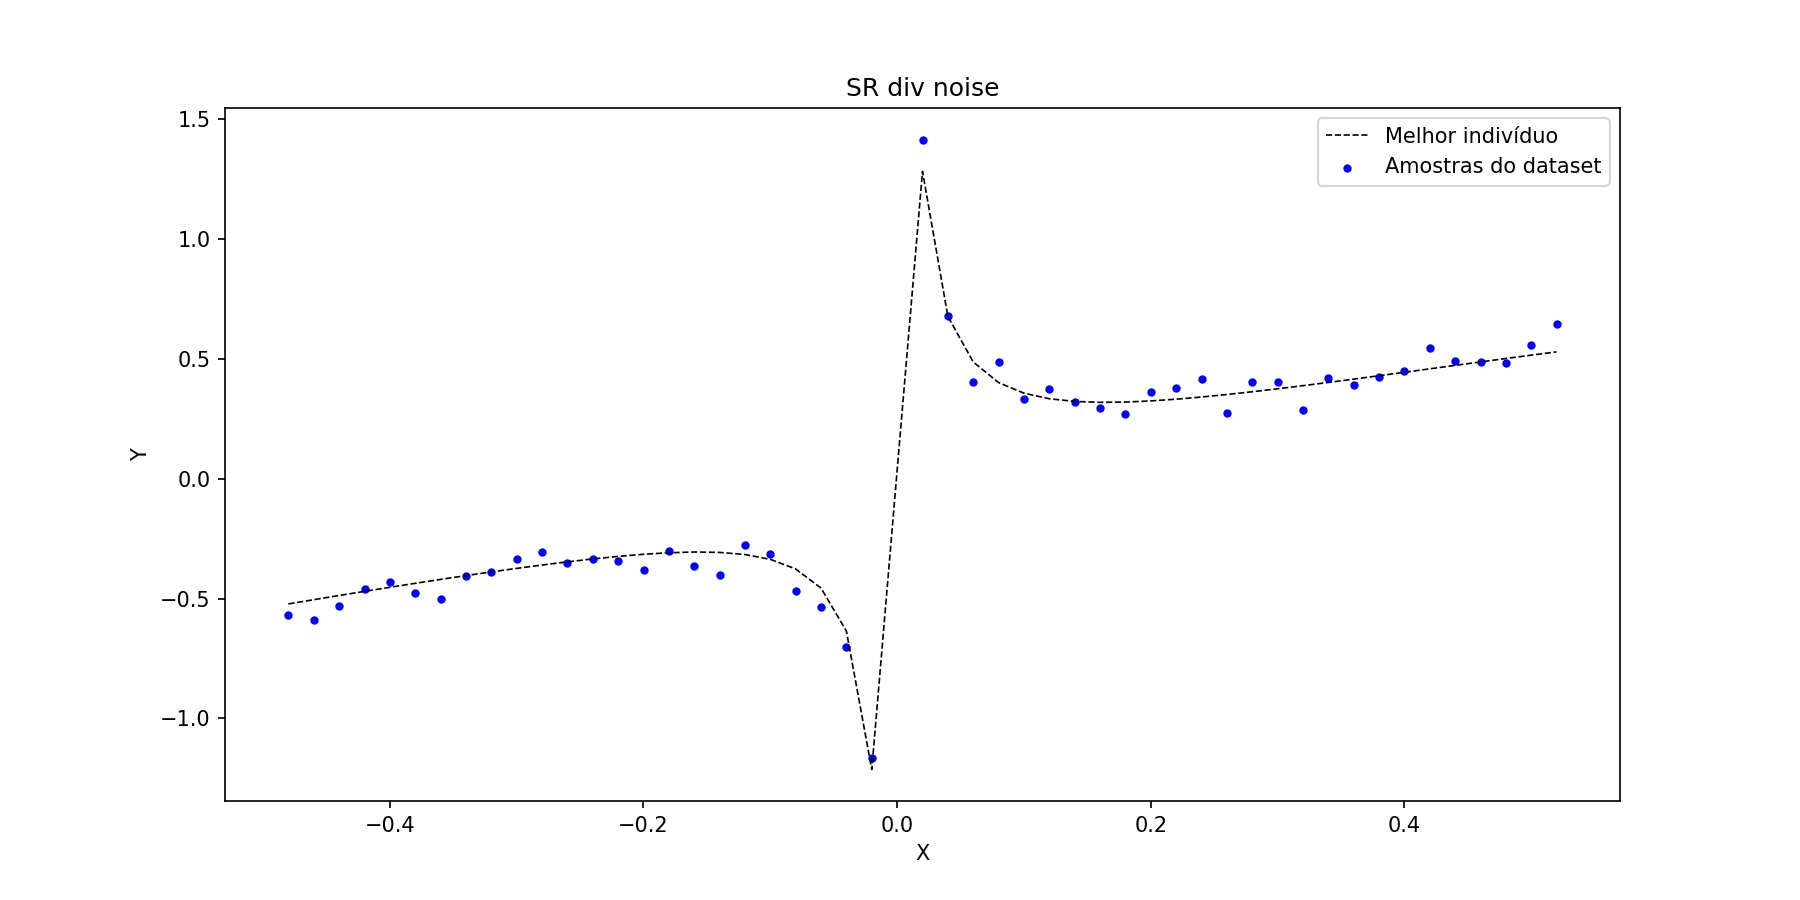
\includegraphics[width=\textwidth]{best_individual_noise}
    \caption{Melhor indivíduo gerado (com ruído)}
    \label{fig:best_sd}
  \end{subfigure}
  \begin{subfigure}[t]{0.5\textwidth}
    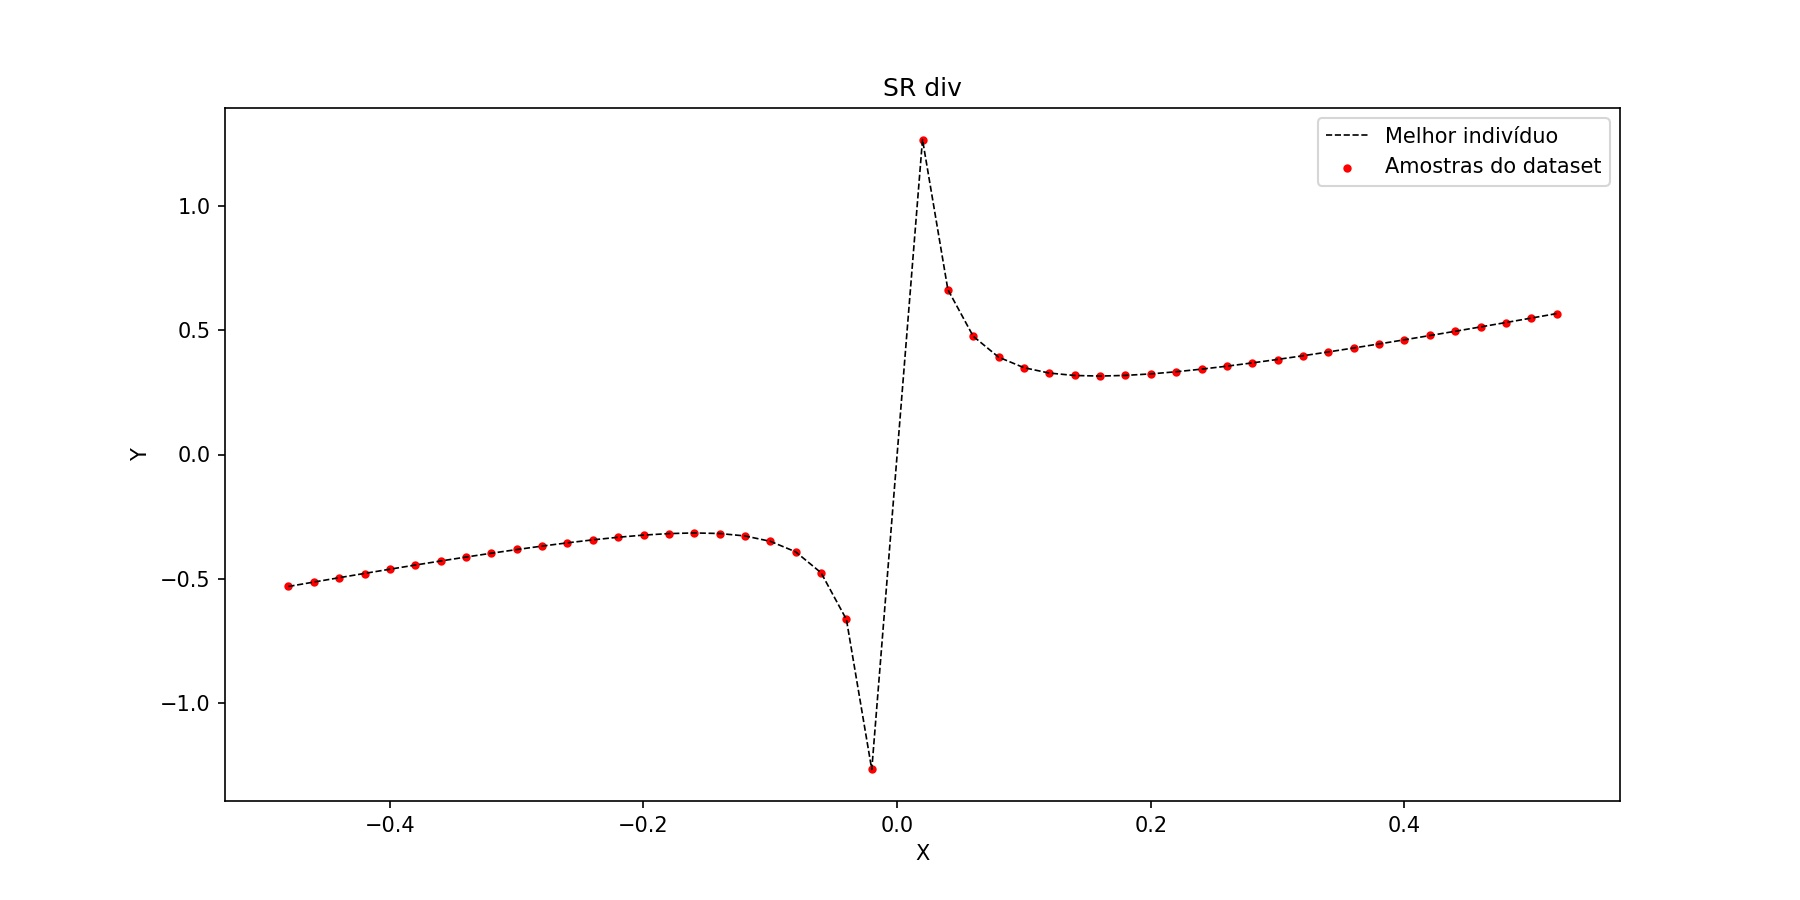
\includegraphics[width=\textwidth]{best_individual}
    \caption{Melhor indivíduo gerado (sem ruído)}
    \label{fig:best_sdn}
  \end{subfigure}
\end{figure}

\subsection{Dataset Real}
Neste experimento, o sistema é testado com um dataset que contêm dados sobre
concreto. Este dataset contêm 9 colunas. Portanto, a regressão utiliza até 8
diferentes variáveis. O procedimento para encontrar o conjunto de parâmetros que
resulta na melhor \textit{fitness} é: \begin{ilist} \item identificar o tamanho
  da população,
\item identificar a probabilidade de mutação e de \textit{crossover}, \item
  identificar o tamanho do torneio (k) e
  \item identificar o efeito da ausência de eletismo \end{ilist}.

Para executar os experimentos, quando um deles é variado, os demais permanecem
constantes. Os valores iniciais dos parâmetros são: 8 variáveis independentes,
profundidade da árvore igual 7, limite de gerações igual a 100, eletismo ativado,
probabilidade de \textit{crossover} igual a 90\%, probabilidade de mutação igual
a 5\%, probabilidade de reprodução igual a 5\%,
10 funções, 5 operadores e constantes variando de -10 a +10.

Para identificar o tamanho da população, os seguintes valores foram testados:
50, 100, 300 e 500. Espera-se que com o aumento do tamanho da população haja um
aumento da qualidade da \textit{fitness}, pois há mais \textit{exporation} e
\textit{explotation} do que com uma população menor. Os resultados para cada
população pode ser vista na
\hyperref[fig:concrete_pop_sz_e]{Figura~\ref*{fig:concrete_pop_sz_e}}. A melhor
\textit{fitness} é atingida quando o tamanho da população é máximo, o que é
justificado pelo argumento apresentado acima. A população pequena não explora o
espaço de soluções, por isso a \textit{fitness} (erro médio absoluto) não reduz
significativamente, ao passo que, quando a população aumenta o espaço explorado
também aumenta e soluções melhores são encontradas. Para os demais experimentos,
o tamanho da população é fixado em 500 indivíduos.

Os próximos parâmetros testados são a probabilidade de \textit{crossover}
($p_c$) e mutação ($p_m$). Os resultados anteriores foram executados com
$p_c=90\%$ e $p_m=5\%$ e são usados como referência para os pares de
probabilidades testados:  $p_c=80\%, p_m=15\%$; $p_c=70\%, p_m=25\%$ e
$p_c=60\%, p_m=30\%$. Conforme citado em diversos trabalhos, em PG, o
\textit{crossover} não possui nenhum signifcado semântico e se comporta
semenhantes a mutação, portanto, diferentemente do GA, a probabilidade de
mutação mais alto deve gerar melhores resultados do que com a probabilidade de
\textit{crossover} elevado. Os resultados dos testes estão presentes na
\hyperref[fig:concrete_pc_pm_e]{Figura~\ref*{fig:concrete_pc_pm_e}}, onde é
possível verificar que a \textit{fitness} atinge o melhor valor quando a
probabilidade de mutação é máximo. Isso se deve ao fato que a mutação leva a
maior \textit{exploration} do espaço de solução, por isso a população gerada com
alta taxa de mutação obtêm \textit{fitness} menores. Para o próximos testes, os
valores $p_c = 70\%$ e $p_m = 25\%$ é mantido.

Outro parâmetro explorado é o tamanho do torneio, isto é, o $k$ do método de
seleção $k$-\textit{tournament}. O valor de $k$ tem impacto na pressão seletiva
da população. Isso ocorre pois conforme o tamanho do torneio aumenta, mais
indivíduos são selecionados para o torneio, aumentando a probabilidade de que
indivíduos que estão nas posições iniciais no torneio (os mais bem adaptados;
melhores \textit{fitness}) o que faz com eles sejam seleciodados com maior
frequência do que os que estão nas posições mais inferiores. Os valores testados
para $k$ devem ser proporcionais ao tamanho da população, pois valores muito
pequenos gera indivíduos que não convergem. Os seguintes valores são
experimentados: $k=7$, $k=10$ e $k=13$. Os resutados do experimentos podem ser
vistos na \hyperref[fig:concrete_k_e]{Figura~\ref*{fig:concrete_k_e}}. Os
resultados indicam que o melhor valor para o tamanho do torneio para este caso é
$k=7$, pois gera a melhor \textit{fitness}. Como explicado acima, os valores
maiores tem a convergência rápida inicialmente, porém são conservadores e não
exploram o espaço de solução como os que possuem valores menores. Para os
próximo experimento o valor do tamanho do torneio é mantido em $k=7$.

Por fim, o último parâmetro explorado é a presença ou ausência de eletismo. O
eletismo faz com que a melhor solução encontrada (o indivíduos com a melhor
\textit{fitness}) seja mantido, porém há redução do espaço de busca, pois novas
soluções (indivíduos diferentes) devem competir com indivíduos que atingiram um
mínimo (ou máximo) local. O eletismo também pode interferir nos efeitos da
mutação e cruzamento geral da população, pois quando dois indivíduos são
cruzados ou um indivíduo é mutados, o decendente concorre implicitamente com os
pais para a próxima geração. Isso faz com que apenas mutações e cruzamentos que
melhorem a \textit{fitness} da população sejam mantidas. Os resultados da
presença ou ausência de eletismo estão presentes na
\hyperref[fig:concrete_e]{Figura~\ref*{fig:concrete_e}}. Os resultados comprovam
o que foi citado acima e a ausência de eletismo gerou indivíduos com melhores
soluções.

Em resumo, os melhores indivíduos são gerados quando o tamanho da população é
500, a probabilidade de \textit{crossover} é $70\%$, a probabilidade de mutação
é $25\%$, o tamanho do torneio é $7$ e a presença do eletismo está
desativada. Esse fatores indicam que o elemento fundamental para encontrar as
melhores solução está no \textit{exploration}, em contraste com o
\textit{explotation}.
 
\begin{figure}[h]
  \caption{Resultados da \textit{fitness}}
  \label{fig:concrete_fitness}
  \begin{subfigure}[t]{0.5\textwidth}
      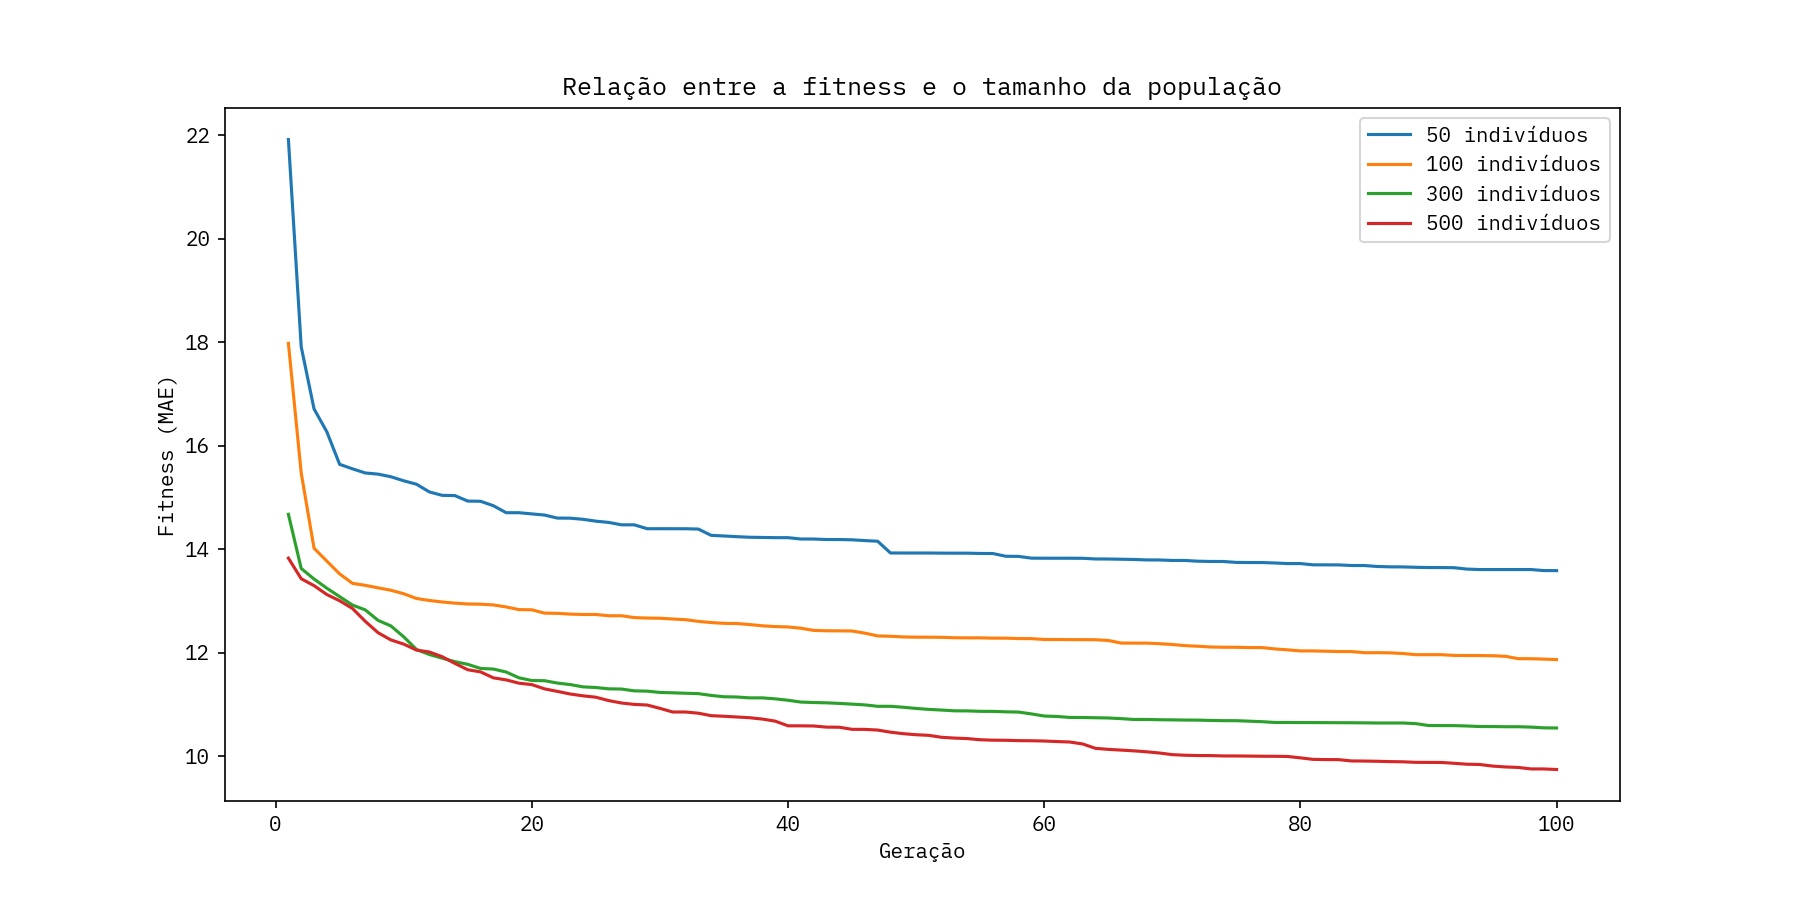
\includegraphics[width=\textwidth]{concrete_pop_sz_e}
      \caption{Tamanho da população}
      \label{fig:concrete_pop_sz_e}
    \end{subfigure}
    \begin{subfigure}[t]{0.5\textwidth}
      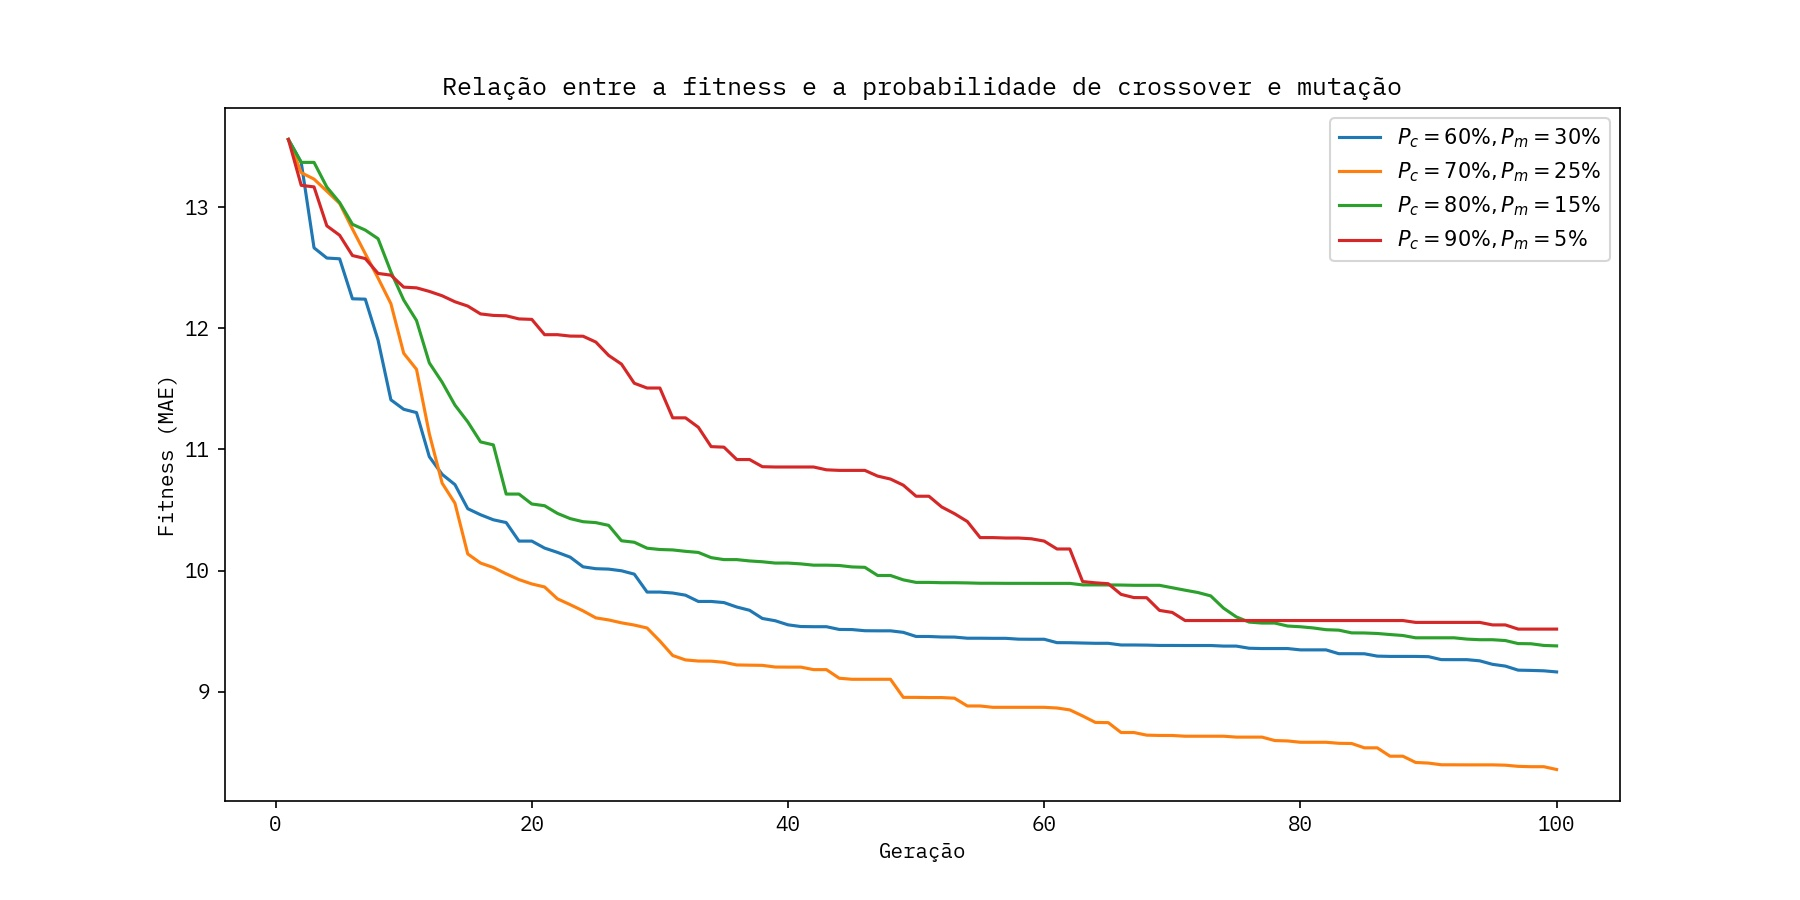
\includegraphics[width=\textwidth]{concrete_pc_pm_e}
      \caption{Probabilidade de \textit{crossover} e mutação}
      \label{fig:concrete_pc_pm_e}
    \end{subfigure}
    \begin{subfigure}[t]{0.5\textwidth}
      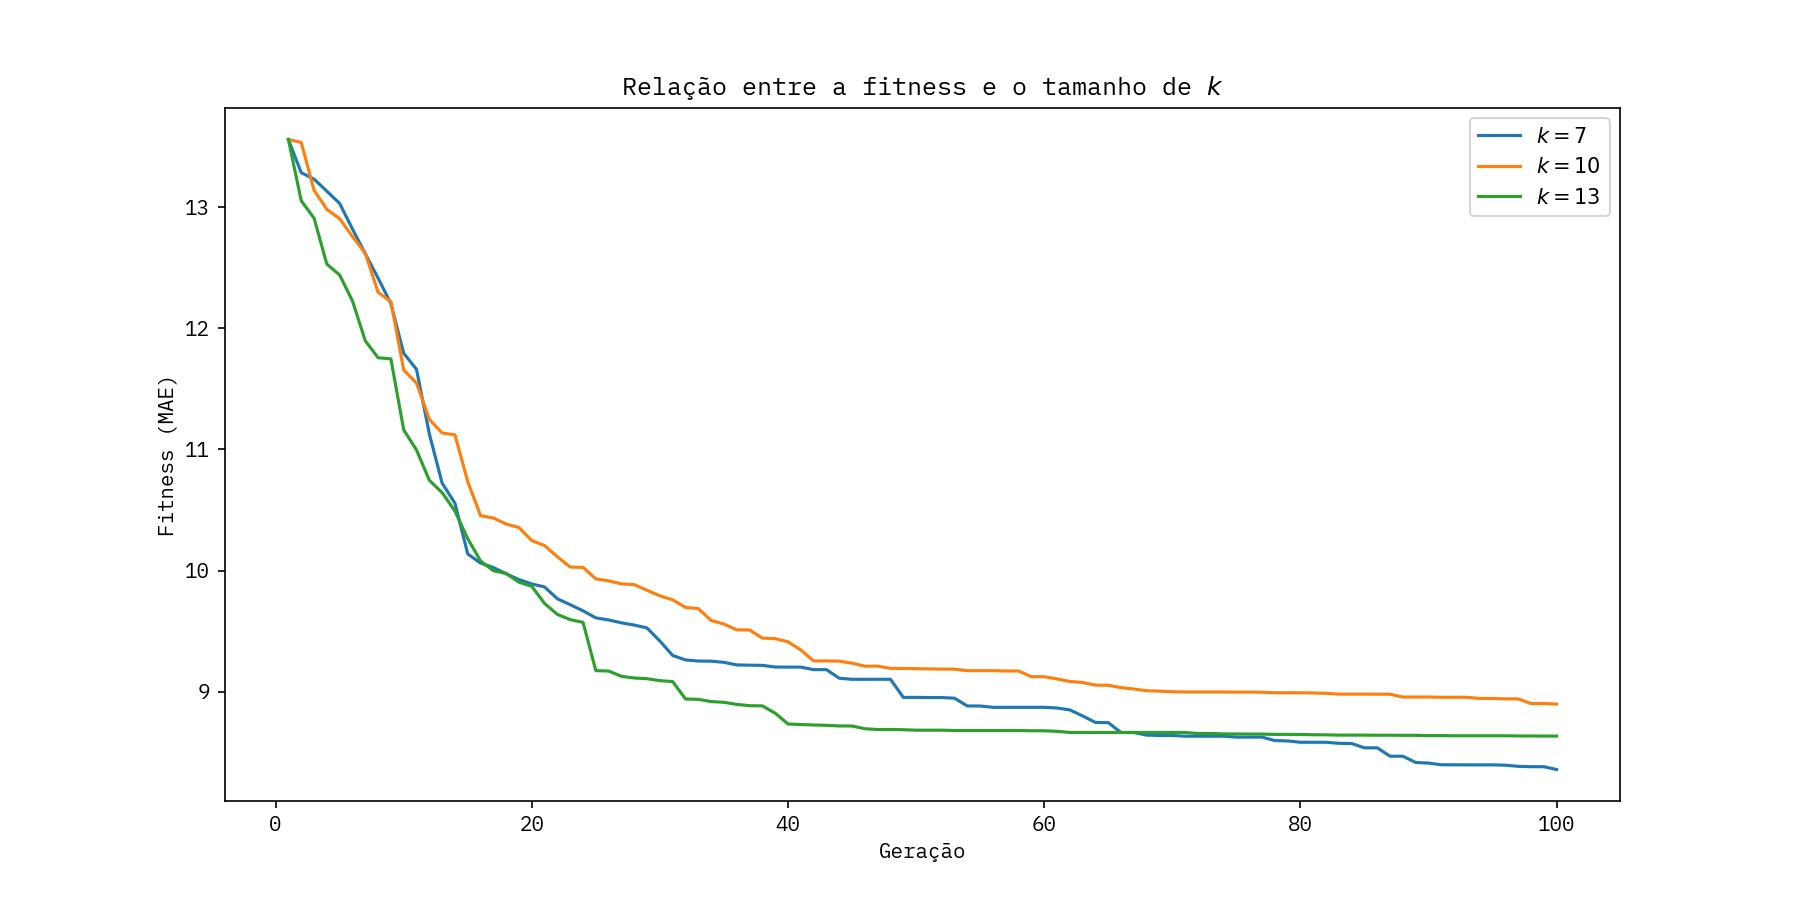
\includegraphics[width=\textwidth]{concrete_k_e}
      \caption{Tamanho do torneio}
      \label{fig:concrete_k_e}
    \end{subfigure}
    \begin{subfigure}[t]{0.5\textwidth}
      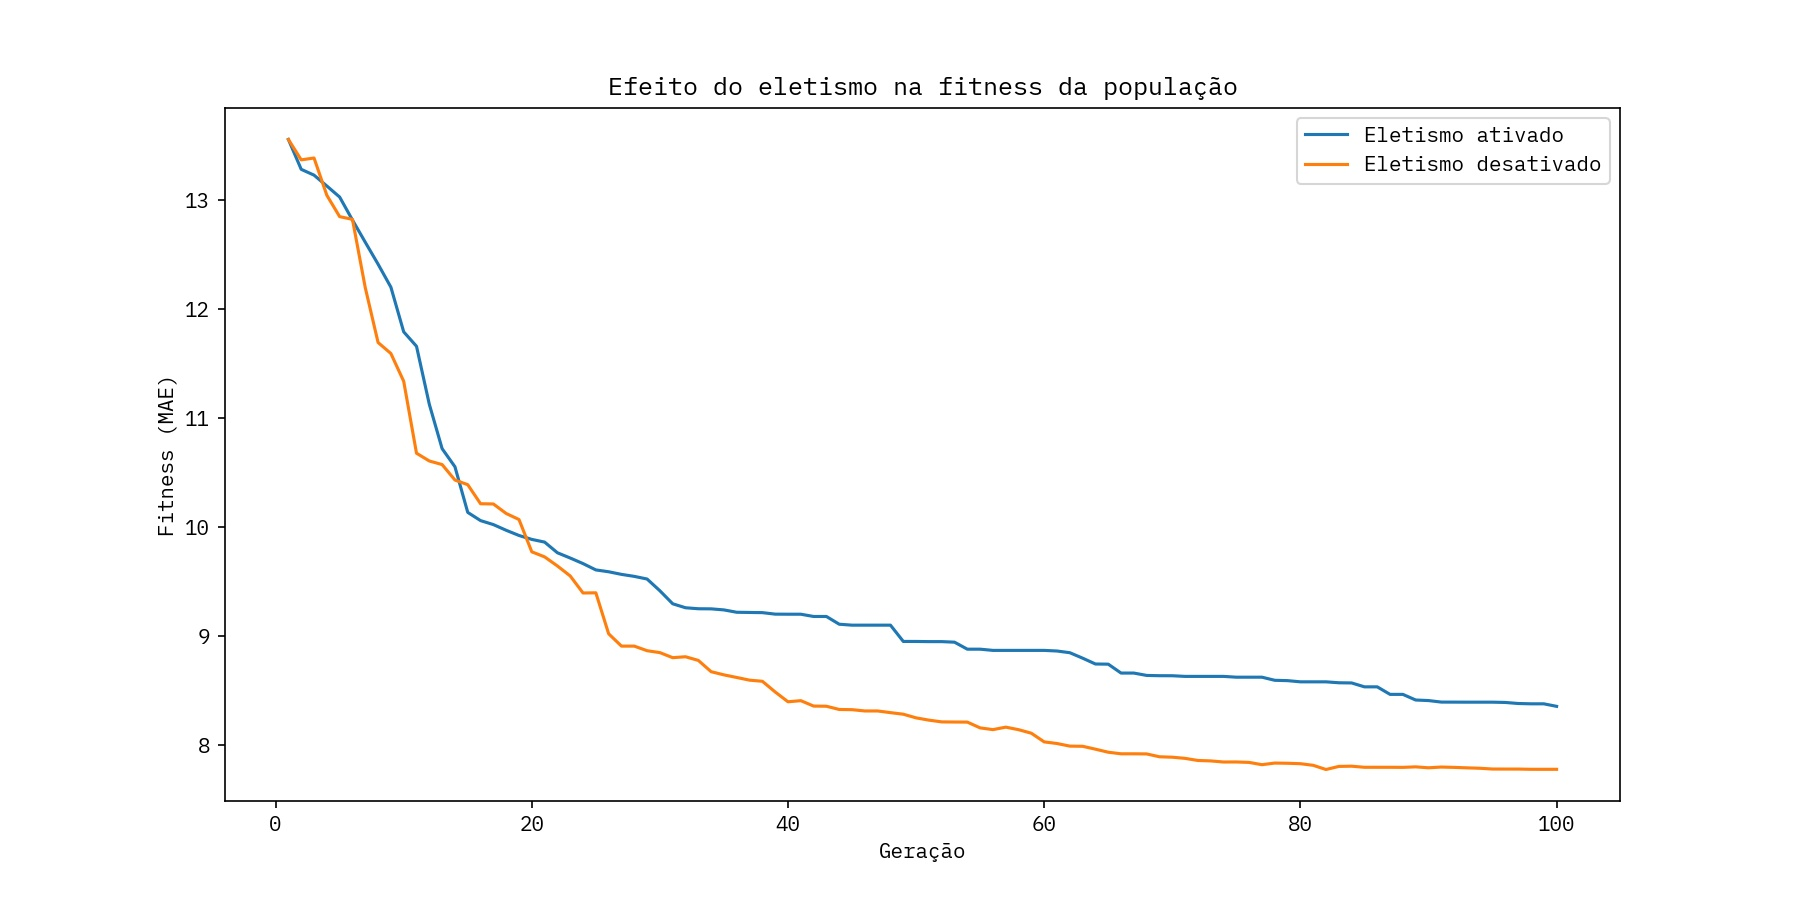
\includegraphics[width=\textwidth]{concrete_e}
      \caption{Efeito do eletismo}
      \label{fig:concrete_e}
    \end{subfigure}
\end{figure}

\section{Conclusão}
Os resultados demonstram a importância no balanceamento dos parâmetros na busca
por soluções ótimas e na importância entre dois fatores que competem entre si:
\textit{exploration} e \textit{explotation}. Os parâmetros que aumentam um
desses fatores faz com que o outro diminua e vice-versa. Portanto, é importante
encontrar o equilíbrio entre eles.

Em termos de implementação, o sistema desenvolvido é robusto e altamente
flexível, pois permite aos usuários definirem novas funções e operadores em
apenas uma linha de código. Outros fatores que podem ser alterados são a
profundidade da árvore, método de geração, método de seleção, métrica de erro,
quantidade de variáveis independentes, tipo de mutação (sub-árvore ou mutação de
ponto), entre outros.

Por fim, algumas melhorias podem ser incorporadas nas próximas versões, como
plotagem da \textit{fitness} em tempo-real, ajuste de parâmetros durante a
execução do algoritmo, ajustar a probabilidade dos operadores e funções de
acordo com os resultados obtidos das soluções que os utilizam, isto é, uma
função que faz com que os indivíduos tenham \textit{fitness} de baixa qualidade
devem ser selecionadas com menos frequência do que as que geram \textit{fitness}
de melhor qualidade.


\bibliographystyle{plainnat}
\bibliography{bibliography}
\end{document}
